\chapter{Desenvolvimento de aplicativos móveis} \label{referencialteorico} 

Nesta seção, serão apresentadas semelhanças e diferenças, vantagens e desvantagens do desenvolvimento nativo em relação ao \textit{cross-plataform}, 
bem como serão descritas as arquiteturas das plataformas \textit{iOS} e \textit{Android}, duas das plataformas mais conhecidas e utilizadas atualmente para desenvolvimento nativo, 
e do \textit{Ionic Framework}, usado para desenvolvimento multiplataformas e \textit{frameworks} necessários para o correto funcionamento do \textit{Ionic}.

%aqui serão descritos as diferencas sucintamente enre nativo e cross
%explicar as diferencas
% Referencias boas para leitura
% http://www.teclogica.com.br/blog/desenvolvimento-para-dispositivos-moveis-nativo-x-cross-platform/ 
% http://pt.slideshare.net/suelengc/nativo-vs-crossplataform
% https://www.ibm.com/developerworks/community/blogs/ctaurion/entry/desenvolvimento_de_apps-parte_2_hibrido_nativo_ou_web?lang=en
% http://blog.concretesolutions.com.br/2016/03/nativo-x-hibrido/
% http://martinfowler.com/articles/multiMobile/#cost

\section{Desenvolvimento Nativo} \label{desenvolvimentonativo}

nativo 


\section{Desenvolvimento \textit{Cross-platform}} \label{desenvolvimentomulti}

multi


\section{iOS} \label{ios}

O sistema operacional \textit{iOS} foi lançado juntamente com o primeiro \textit{iPhone} criado em Janeiro de 2007 e 
funciona como uma interface entre as aplicações desenvolvidas pelos programadores (\textit{apps}) e o \textit{hardware} 
dos dispositivos (\textit{iPhone}, \textit{iPad}, \textit{iPod}). Dessa forma, a comunicação com o \textit{hardware} do dispositivo se dá 
por meio de um conjunto bem definido de interfaces do sistema, o que facilita o desenvolvimento de \textit{apps} 
que funcionam corretamente entre os variados tipos de \textit{hardware} dos dispositivos da Apple. 

Como recomendação, a Apple explica que deve-se preferir o uso de camadas mais elevadas, pois as camadas de 
mais alto nível possuem abstrações orientadas à objeto de funcionalidades das camadas mais baixas. Isso 
torna o desenvolvimento mais fácil, pois reduz a quantidade de código que deve ser criado e mantém funcionalidades 
complexas das camadas mais baixas encapsuladas por meio das interfaces. No entanto, não há problema em usar 
funcionalidades presentes nas camadas mais baixas, se essas não estiverem disponíveis por meio de abstrações nas 
camadas superiores. 

A maioria das interfaces disponíveis para uso são disponibilizadas por meio de \textit{frameworks}, 
que são diretórios, que podem ser adicionados ao projeto no \textit{Xcode}, contendo \textit{DSL's} e os recursos necessários como, 
imagens, aplicativos auxiliares e arquivos \textit{header}, para o \textit{framework} funcionar corretamente.

\subsection{Arquitetura \textit{iOS}} \label{arc-ios-section}
Sua arquitetura é baseada nas camadas listadas, conforme a Figura~\ref{fig:arc-ios} a seguir.
 
\begin{figure}[H]
  \centering
    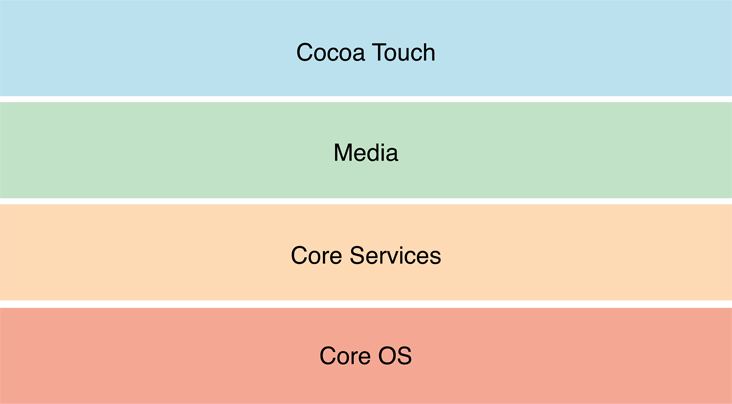
\includegraphics[width=0.5\textwidth]{arc-ios}
    \caption[Arquitetura iOS]{ Arquitetura iOS. Fonte: REFERENCIAR A Apple CORRETAMENTE.}
	\label{fig:arc-ios}
\end{figure}

As camadas do \textit{iOS} são explicadas com mais detalhes a seguir.
 
\begin{itemize}
	\item A camada \textit{Cocoa Touch} é a camada mais alto nível onde são fornecidos serviços básicos de interação 
    com o usuário como entrada baseada em toques e notificações \textit{Push} e outras tecnologias necessárias para
     melhorar a experiencia do usuário como multitarefas, Continuidade (\textit{Handoff}) e \textit{AirDrop}, além de \textit{frameworks} 
     de alto nível que permitem acesso a funcionalidades do sistema como \textit{AddressBook} para contatos, \textit{EventKit} 
     para eventos relacionados ao calendário e \textit{MapKit} para mapas.
	\item A camada logo abaixo da \textit{Cocoa Touch} é a camada \textit{Media} que contém tecnologias e \textit{frameworks} necessários 
    para a implementação de experiências multimídia com áudio, vídeo e gráficos.
	\item A próxima camada, logo abaixo da camada \textit{Media}, é a camada \textit{Core Services}. Essa camada está mais próxima 
    do \textit{hardware} e portanto possui acesso a funcionalidades de mais baixo nível como localização, telefonia, \textit{threads} 
    e \textit{SQLite}. Aqui residem dois dos \textit{frameworks} mais importantes do \textit{iOS} que são o \textit{Foundation} e o \textit{Core Foundation}, 
    ambos relacionados com o gerenciamento de dados e alguns serviços e definem todos os tipos básicos de dados que 
    todos os \textit{apps} usam, como por exemplo, coleções, \textit{strings}, data e hora, \textit{sockets} e \textit{threads}.
	\item A última camada é a camada \textit{Core OS}, na qual as funcionalidades de mais baixo nível são construídas e 
    provavelmente utilizadas por outros \textit{frameworks} em outras camadas. Se a aplicação possui requisitos de segurança 
    ou comunicação com acessórios externos mais complicados, é possível usar as funcionalidades dessa camada.
\end{itemize}

\section{Android} \label{android}

O sistema operacional \textit{Android} foi criado pela \textit{start-up} homônima Android Inc. em outubro de 2003. Em agosto de 2005 foi adquirida pela empresa Google, que lançou
em novembro de 2007, juntamente com a OHA, o sistema \textit{Android}, \textit{open-source} e baseado no \textit{kernel} do Linux. Uma semana depois, foi liberada a primeira versão do \textit{SDK} para \textit{Android}.
O sistema foi concebido originalmente para camêras fotográficas, no entanto, foi percebido por seus criadores um mercado maior no ramo da telefonia e desviou-se o 
foco para \textit{smartphones}, competindo diretamente como Symbian e Windows Mobile.

\subsection{Arquitetura \textit{Android}} \label{arc-android-section}

A arquitetura Android é baseada nas camadas apresentadas na Figura~\ref{fig:arc-android} e são explicadas com mais detalhes a seguir.

\begin{itemize}
%http://source.android.com/devices/index.html <- Fonte principal
%traduzir e parafrasear

    \item A camada mais elevada é a \textit{Application Framework}, onde as aplicações construídas pelos desenvolvedores são instaladas.
    \item A camada logo a abaixo da \textit{Application Framework} é a \textit{Binder IPC Proxies}, onde \textit{IPC} significa \textit{Inter-Process Comunication}.
    É a camada que faz uma ponte entre as aplicações instaladas na camada superior com a próxima camada, a \textit{System Services}. É uma interface que permite que \textit{API's}
    de alto nível interajam com serviços do sistema que residem na camada abaixo dela. 
    \item Abaixo da \textit{Binder IPC Proxies} fica a \textit{System Services}, que , por meio de módulos, permite acesso a \textit{hardwares} específicos. Cada serviço presente nessa camada,
    foi desenvolvido para gerenciar um componente específico, como busca e notificações. Os serviços foram divididos em duas categorias, \textit{Media} e \textit{System}, explicadas a seguir.
    \begin{itemize}
        \item \textit{Media Server}: são os serviços responsáveis por gerenciar conteúdos de mídia como gravação e reprodução de audio e vídeo. 
        \item \textit{System Server}: são serviços responsáveis por gerenciar os demais tipos de serviço do sistema como notificações e \textit{windows}.
    \end{itemize}
    \item Abaixo da camada \textit{System Services} fica a camada \textit{HAL} que permite que fornecedores de \textit{hardware} criem interfaces e \textit{drivers} para os \textit{hardwares} que
    ele oferecem. Com isso, é possível criar novas funcionalidades e implementá-las sem afetar o resto das camadas do sistema.  
    \item A camada mais baixa é a \textit{Linux Kernel} que é uma versão do \textit{kernel} do Linux com algumas modificações como uma gerenciamento de memória mais avançados e próprio para dispositivos 
    móveis e funcionalidades para dispositivos embarcados. 
    
\end{itemize}

\begin{figure}[h]
  \centering
    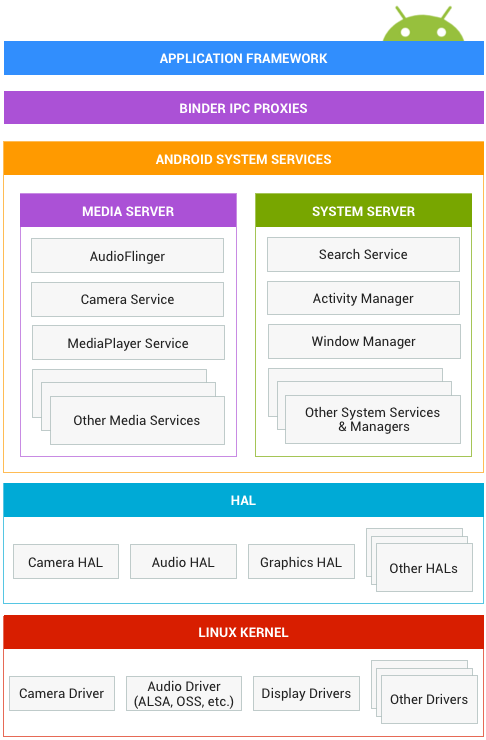
\includegraphics[width=0.35\textwidth]{arc-android}
    \caption[Arquitetura Android]{ Arquitetura Android. Fonte: REFERENCIAR A Google CORRETAMENTE.}
	\label{fig:arc-android}
\end{figure}

\section{PhoneGap e Cordova} \label{subsec:phonegap}

\textit{PhoneGap} é um \textit{framework} para desenvolvimento de aplicativos híbridos, criado pela empresa Nitobi. 
Após a empresa ser comprada pela Adobe Systems Inc. o \textit{PhoneGap} teve seu código doado para a Apache Software Foundation 
para garantir que outras empresas pudessem contribuir, já que muitas empresas já conheciam as licenças da Apache.


Como o \textit{PhoneGap} é uma marca registrada de propriedade da Adobe, na Apache teve seu nome alterado para Cordova.
Tanto o \textit{Apache Cordova} quanto o \textit{Adobe PhoneGap}, são gratuitos e \textit{open sources}, no entanto, o 
\textit{PhoneGap} possui um ambiente integrado com serviços da Adobe como o \textit{PhoneGap Build}, por exemplo.
 
\textit{Cordova} permite que aplicações não nativas tenham acesso a funcionalidades nativas do dispositivo como sensores, 
contatos e câmera. No entanto, o Cordova apenas consegue fazer um aplicativo criado em 
\textit{HTML} rodar como se fosse nativo em um dispositivo com \textit{Android} e \textit{iOS}, mas não consegue 
imitar a usabilidade e aparência dos dispositivos nativos. 


Para preencher essa lacuna, outros \textit{frameworks} foram criados em cima do Cordova como um complemento, 
provendo bibliotecas \textit{HTML} e \textit{CSS} para a 
criação de um \textit{front-end} que se aproxime o máximo possível da usabilidade e experiência de usuário de 
aplicações móveis nativas.

O \textit{Cordova} possui muitos plugins para poder acessar funcionalidades específicas do aparelho em que está sendo 
executado. Esses devem ser instalados no projeto do aplicativo via \textit{CLI}. 

A fim de se evitar confusões em relação aos nomes dados ao \textit{PhoneGap} e ao \textit{Cordova}, pode-se entender o \textit{PhoneGap} 
como uma distribuição do \textit{Apache Cordova}, mantido pela Adobe Systems Inc. 

%https://www.quora.com/What-is-the-difference-between-PhoneGap-and-Cordova-and-why-would-I-select-one-over-another
%http://luisvasconcellos.com/2015/04/06/apps-hibridas-com-cordova-e-ionic.html
%https://www.quora.com/What-is-the-difference-between-Cordova-and-Ionic
%https://en.wikipedia.org/wiki/Apache_Cordova
%http://cordova.apache.org/docs/en/latest/guide/overview/

\section{AngularJS} \label{subsec:angularjs}

\textit{HTML} é a principal linguagem de marcação para a criação de páginas \textit{web}. No entanto, os conteúdos exibidos são estáticos e o \textit{HTML} não fornece suporte para conteúdos dinâmicos.
\textit{AngularJS} é um \textit{framework open source}, mantido pelo Google, que permite extender a sintaxe do \textit{HTML} para poder criar páginas \textit{web} com conteúdos dinâmicos.


Com ele é possível utilizar \textit{tags} não nativas do \textit{HTML} para gerenciar conteúdos que ainda não foram dispostos na tela, ou seja, o usuário faz uma ação por meio da interface gráfica, 
o AngularJS interpreta a ação e faz uma requisição para o servidor pedindo apenas o conteúdo necessário, que é diferente do que já está sendo mostrado para o usuário. 
O servidor retorna o conteúdo específico e o AngularJS apresenta o novo conteúdo inserindo-o corretamente junto com o antigo já mostrado.


Foi projetado para criação de \textit{SPA's} e com isso faz com que as páginas sejam mais rápidas, visto que, apenas é carregado o conteúdo que precisa ser mostrado, 
deixando outros conteúdos para serem carregados dinâmicamente depois, de acordo com as interações do usuário.   

\section{Ionic} \label{ionic}
%http://blog.ionic.io/how-2015-went-for-ionic/
\textit{Ionic} é um \textit{framework} gratuito e \textit{open source} para desenvolvimento de aplicativos híbridos utilizando tecnologias 
\textit{web} como \textit{HTML}, \textit{CSS} e \textit{JavaScript} otimizadas para dispositivos móveis. 


Foi criado pela empresa Drifty Co. em 2013 com base na necessidade que seus clientes apresentavam de criarem \textit{apps}. 
Foi projetado para ser muito performático e funcionar com padrões e tecnologias \textit{web} modernas. 


Criado sobre os \textit{frameworks} \textit{Cordova} e \textit{AngularJS}, com apenas um código é possível criar aplicativos para várias 
plataformas como \textit{iOS} e \textit{Android}, por exemplo, dentre outras. O \textit{Ionic} conta ainda com um conjunto de ferramentas para auxiliar 
no desenvolvimento dos aplicativos.

\subsection{Arquitetura de um projeto Ionic} \label{subsec:arc-ionic}

Um projeto Ionic segue a seguinte arquitetura...


Um projeto Ionic segue a seguinte estrutura de diretorios...

\subsection{Ferramentas de Apoio} \label{subsec:ferramentasapoio}

O \textit{Ionic} provê além do \textit{HTML} e \textit{CSS} otimizado para dispositivos móveis, uma série de ferramentas de 
apoio que fornecem velocidade e facilidade no desenvolvimento de aplicativos híbridos. Essas ferramentas são listadas a seguir 
com uma breve explicação do que cada uma pode fazer.

\begin{itemize}

    \item \textbf{Ionic Framework}: É o \textit{framework front-end} para criação de aplicativos híbridos com tecnologias \textit{web} construído em cima
    do \textit{Apache Cordova}. Facilita a criação de aplicativos com interface gráfica e interações muito semelhantes aos dispositivos nativos, de modo que 
    a experiência de usuário não seja diferente no uso de uma aplicação nativa e multiplataforma. 
    
    \item \textbf{Ionic Creator}: Com essa ferramenta \textit{on-line} é possível criar protótipos funcionais utilizando \textit{drag and drop}
    , que podem ser executados em dispositivos ou simuladores, e depois exportar o projeto criado para a 
    inserção de lógicas de negócio. Ela é gratuita para teste, ou seja, é possível criar um protótipo e fazer o \textit{download}
    do código para continuar o desenvolvimento, no entanto, no momento em que este trabalho foi conduzido, só era possível
    fazer a pré-visualização em dispositivos reais para usuários pagantes.
    
    \item \textbf{Ionic Lab}: É uma ferramenta \textit{desktop} para testar o projeto que está sendo criado com o \textit{Ionic}. Nela é possível
    executar o projeto em templates prontos de \textit{iOS} e \textit{Android}, rodar os simuladores de cada plataforma,
    gerenciar plugins do \textit{Cordova} e ver um console com \textit{logs} relativos à execução do projeto. Encapsula o \textit{CLI} do \textit{Ionic} com uma interface gráfica simples
    e intuitiva.
    
    \item \textbf{Ionic Playground}: É uma ferramenta \textit{on-line} para criar e testar códigos \textit{HTML}, \textit{CSS} e \textit{JavaScript} 
    já integrado com a plataforma \textit{AngularJS}. Nela é possível editar códigos nas três linguagens citadas e ver em tempo real as alterações 
    feitas aparecerem dentro de um \textit{template} de dispositivo móvel, sem a necessidade de salvar, compilar ou executar o projeto e sem ter que 
    configurar o ambiente necessário para o desenvolvimento. 
    
    \item \textbf{Ionic View App}: É um aplicativo disponível para as plataformas \textit{iOS} e \textit{Android} onde é possível testar o 
    aplicativo criado no \textit{Ionic} diretamente em um dispositivo real como se fosse nativo. É possível compartilhar os projetos criados para serem
    testados por clientes e testadores sem a necessidade de passar pelas lojas de aplicativos de cada plataforma. É semelhante ao serviço 
    \textit{Testflight} da Apple para testar aplicativos, ainda em desenvolvimento, e receber \textit{feedbacks} dos clientes e testadores que o testarem.
    
    \item \textbf{Ionic Platform}: É a plataforma \textit{on-line} do \textit{Ionic} que possui serviços de \textit{back-end} em nuvem para análise de dados de uso,
     usuários, configuração de \textit{Push Notifications}, criação dos pacotes nativos e dar \textit{deploy} nas aplicações criadas sem a necessidade de
     resubmeter o aplicativo para as respectivas lojas. 
     
\end{itemize}